\chapter{Learning from complex vehicle model}
\label{cha:Tracking_MPC}

%Plot simulink model en duidt de blokken aan die zullen worden ingevuld. Hier gaat dieper in gegaan worden in de volgende hoofdstukken. 

Because the non-linear bicycle model makes abstraction of dynamics that are applicable in a real vehicle, a more complex model is introduced in order to improve the reality factor of the simulations. In order to achieve this the $15$ degrees of freedom amesim model as can be seen in Figure \ref{fig:Amesim}, is provided by Siemens. The parameters of this model are tuned by the company in order to behave similar to a testcar they are currently using. The model has as inputs the amount of throttle, braking and a steerwheelangle.  

\begin{figure}[h!]
	\centering
	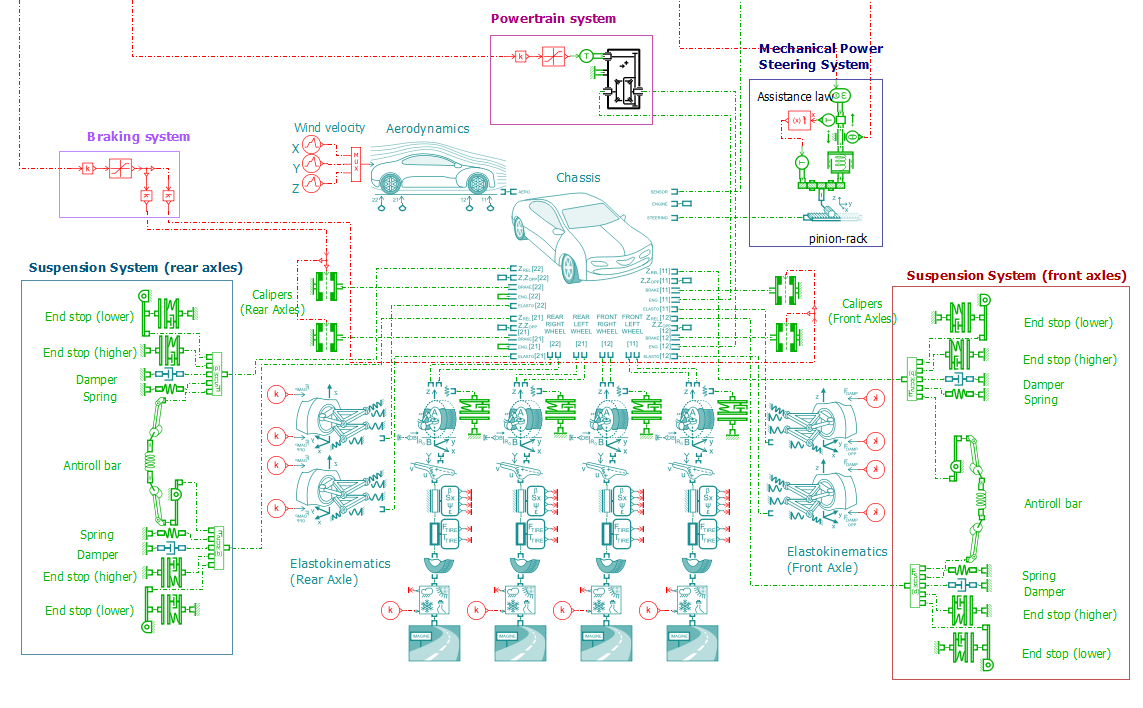
\includegraphics[width=1.0\textwidth]{Amesim.PNG}
	\caption{The 15 dof amesim model with as inputs the amount of throttle, braking and steerwheelangle.}	
	\label{fig:Amesim}
\end{figure}

The Amesim model serves as a black box and no direct dynamic equations are available 
to include in \ref{opt:basic_opti_w} as was done with the non-linear bicycle model \ref{eq:bicycle_model_eqmotion}. Therefore a path is planned with the simpler non-linear bicycle model and afterwards a model predictive control tracking algorithm is applied on the Amesim model in order to follow the reference. The working principles of a MPC is discussed in \ref{s:MPC_e}. Diagram \ref{fig:complex_learning} shows the flow of handlings that is done during learning with the Amesim model.

\begin{figure}[h!]
	\centering
	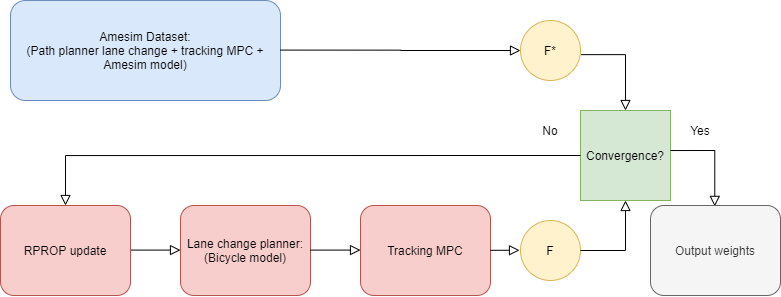
\includegraphics[width=1.1\textwidth]{complex_learning_diagram.PNG}
	\caption{The flow of learning with the Amesim model.}	
	\label{fig:complex_learning}
\end{figure}

As is described in Diagram \ref{fig:complex_learning} the feature vector $\bm{F}(\bm{r})$ is also calculated based on the Amesim model and used in the convergence block to calculate the estimation of the gradient by $\pdv{\bm{F}}{\bm{\theta}} = \bm{F}_{obs} - \bm{F}(\bm{r}_{expected})$. The reason for this is to avoid to integrate the vehicle mismatch between the non-linear bicycle model and the Amesim model into the learned path. This concretely means that it otherwise is possible that even when the learning algorithm is capable to match the feature vectors $\bm{F}(\bm{r})$ and  $\bm{F}^*(\bm{r})$, coming form two different vehicle models, the learned kinematic signals of the bicycle model will not represent the observations accurate enough. In order to check this, table \ref{tab:comparinson_models} \footnote{Note that the feature values of the bicycle model are slightly different values than the ones in table \ref{tab:GD_local_test}. This is because in the previous table the time limit was set on $30 \hspace{1mm}s$ and here time limit is $30 \hspace{1mm}s$. This is done to have a better useable time discretization of $0.025\hspace{1mm}s$ to input to the Amesim model.} shows the difference of feature values for a lane change $V_0:22.22\hspace{1mm}\frac{m}{s},\hspace{1mm} L:3.47\hspace{1mm}m$ generated with the non-linear bicycle model and afterwards tracked with the Amesim model.\\

\begin{table}[h!]
	\centering
	\begin{tabular}{@{}llr@{}} \toprule
		Feature Value    & Bicycle model & Amesim model\\ \midrule
		Nr.1       		 & 5.28e-8    & 3.33e-7 \\
		Nr.2       		 & 0.37       & 0.38  \\
		Nr.3       		 & 1.41e-7    & 1.20e-4 \\
		Nr.4       		 & 0.57       & 0.49  \\
		Nr.5       		 & 1.89e-6    & 9.40e-6 \\
		Nr.6       		 & 30.99      & 31.05\\ \bottomrule
	\end{tabular}
	\caption{This table shows the feature values obtained of a lane change $V_0:22.22\hspace{1mm}\frac{m}{s},\hspace{1mm} L:3.47\hspace{1mm}m$ for respectively the Bicycle and Amesim model.}
	\label{tab:comparinson_models}
\end{table}

As can be seen the features of the reference produced by the bicycle model are almost the same as the ones that are retrieved from the Amesim model during the application of the tracking MPC. However not all kinematic signals give an accurate match as is described in Appendix \ref{app:D} and further discussed in section \ref{s:tracking_mpc}. 

This chapter also gives an answer on the question if the estimate of the gradient $\pdv{\bm{F}}{\bm{\theta}}$ by $ \bm{F}_{obs} - \bm{F}(\bm{r}_{expected})$ is still sufficient in order to match the learned and observed feature values in section \ref{s:complex_learning_results}.\\

\section{Tracking MPC} 
\label{s:tracking_mpc}
To be able to integrate the Amesim model in the learning process in an adequate manner, good tracking is desirable for the important features that determine the lane change planning. For the lane change maneuver looked at in this thesis, a good tracking is therefore wanted for: $y(t), a_y(t)$ and $j_y(t)$.

\subsection{MPC formulation}
The tracking is achieved by making use of the non-linear bicycle model defined with 10 states as defined in \ref{eq:bicycle_model2} inside the OCP formulation given by $\ref{opt:tracking}$ that is called during the MPC loops. The control horizon of the MPC is $N_{MPC}$ and equal to $50$ points which means a control horizon of $1.25 \hspace{1mm}s$ because the reference is sampled with $T_{pl}$ equal to $0.025\hspace{1mm}s$. The parameters of the bicycle model stay the same as the ones listed in \ref{table:vehicel_model_param}. The objective function used is the error function between the reference states and the states visited during the control horizon starting from the current state. In order to define the gap closing constraint, which means connecting the previous states to the next in this multiple shooting formulation, Runge-Kutta integration is embedded in function $I$.  
The first time that the OCP is solved and the current state is not yet outputted by the sensors on the Amesim model, the initial states are set equal to its first reference point. The path constraints can be seen in \ref{eq:F_MPC} and the error function $E(\bm{X}(.),\bm{U}(.))$ that serves as objective is shown in \ref{eq:obj_mpc}.


\begin{equation}\label{opt:tracking}
\begin{aligned}
\min_{\bm{X}(.),\bm{U}(.)} \quad &  E(\bm{X}(.),\bm{U}(.)) \\
\textrm{s.t.} \quad & \bm{X}^{k+1} = I(\bm{X}^{k}, \bm{U}^{k}) & k = [0,\cdots, N_{MPC}-1]\\
& \bm{X}^{0} = \bm{X}_{intitial} \\
& \bm{F}(\bm{X}^{k}) \geq 0	& k = [0,\cdots, N_{MPC}]\\
& \bm{X}^{k}\in \mathbb{R}^{10x1}  & k = [0,\cdots, N_{MPC}]\\
& \bm{U}^{k}\in \mathbb{R}^{2x1} \hspace{3 mm} & k = [0,\cdots, N_{MPC}-1]\\
&  N_{MPC} \in \mathbb{N}
\end{aligned}
\end{equation}

The path constraints shown in \ref{eq:F_MPC} are at first sight not necessary but contribute by decreasing the feasible solution space for the solver in \ref{opt:tracking}. It is checked that these constraints are not binding, which means that the found solution is reachable even if the constraints were removed. 

\begin{equation}\label{eq:F_MPC}
\bm{F} =
\begin{Bmatrix}
-\frac{Width\hspace{1mm}Lane}{2} \leq y^k \leq \frac{3\cdot Width\hspace{1mm}Lane}{2}, & k = [0,\cdots, N_{MPC}] \\
0 \leq x^k, & k = [0,\cdots, N_{MPC}] \\
-\frac{\pi\cdot 5}{180} \leq \psi^k \leq \frac{\pi\cdot 5}{180}, & k = [0,\cdots, N_{MPC}] \\
v_{start}-1 \leq v_x^k \leq v_{start}+1, & k = [0,\cdots, N_{MPC}]
\end{Bmatrix}
\end{equation}\

The error function that serves as the objective of the OCP is given by the following equation.

%\label{eq:obj_mpc}

\begin{multline*} 
objective=W_1(\bm{x}-\bm{ref}_x)^T(\bm{x}-\bm{ref}_x)+W_2(\bm{y}-\bm{ref}_y)^T(\bm{y}-\bm{ref}_y)\\
+W_3(\bm{v}_x-\bm{ref}_{v_x})^T(\bm{v}_x-\bm{ref}_{v_x})+W_4(\bm{v}_y-\bm{ref}_{v_y})^T(\bm{v}_y-\bm{ref}_{v_y})\\+W_5(\bm{\psi}-\bm{ref}_{\psi})^T(\bm{\psi}-\bm{ref}_\psi)
+W_6(\bm{\dot{\psi}}-\bm{ref}_{\dot{\psi}})^T(\bm{\dot{\psi}}-\bm{ref}_{\dot{\psi}})\\ + W_7\dot{\bm{t}}_r^T\dot{\bm{t}}_r+W_8\dot{\bm{\delta}}_s^T\dot{\bm{\delta}}_s + W_9\dot{\bm{a}}_x^T\dot{\bm{a}}_x
\end{multline*}













\subsection{Tracking results}













\section{Learning results with the Amesim model}
\label{s:complex_learning_results}

Diagram \ref{fig:complex_learning} shows in blue the observed path that is generated out of \ref{opt:basic_opti_w} with known weights whereafter the path based on a bicycle model is tracked by a tracking MPC to get the kinematic signals of the $15$ dof Amesim model. From this $\bm{F}^*(\bm{r})$ is calculated which stays constant during whole the learning process.\\

The learning loop shown in red in diagram \ref{fig:complex_learning} start at the lane change planner, where \ref{opt:basic_opti_w} is called with as initial guess of the weights an all one vector. After the planned path that was outputted by the planner is tracked and the feature vector $\bm{F}(\bm{r})$ is calculated, it is checked if the two feature vectors match in the convergence block. If not the difference of the features is taken as an estimate for $\pdv{\bm{F}}{\bm{\theta}}$ and used in the RPROP algorithm in order to generate a new planned path by calling \ref{opt:basic_opti_w}.


\section{Conclusion}

%%% Local Variables: 
%%% mode: latex
%%% TeX-master: "thesis"
%%% End: 